\chapter{Вычислительные эксперименты}
\section{Алгоритм решения}

Для численного решения системы дифференциальных уравнений будем использовать алгоритм Рунге-Кутты \cite{1964calculus} четвертого порядка.

Метод Рунге-Кутты четвертого порядка (RK4) обладает порядком точности \( O(h^4) \), что означает, что ошибка метода уменьшается пропорционально четвертой степени размера шага \( h \). Локальная ошибка на каждом шаге составляет \( O(h^5) \), а глобальная ошибка, накапливаясь после \( N \) шагов, составляет \( O(h^3) \). Это делает метод RK4 более точным по сравнению с методами более низкого порядка, такими как метод Эйлера и метод Рунге-Кутты второго порядка. Благодаря высокой точности и простоте реализации, RK4 широко используется для численного решения обыкновенных дифференциальных уравнений в различных областях науки и техники.

 Результатом применения метода Рунге-Кутты будут являться три массива значений: массив значений времени и два массива численных значений решения (хищники и жертвы). После этого построим графики решений на координатной и фазовой плоскостях.

\section{Программа для ЭВМ}

В качестве языка программирования для рассчётов и визуализации был выбран Python с использованием библиотек numpy (вычисления) и matplotlib + seaborn (визуализация).

\lstinputlisting[language=Python,
captionpos=t,
]{./listings/main.py} 

\section{Результаты экспериментов}
Построим несколько решений системы с одинаковыми параметрами, но разными начальными условиями, включая точку равновесия.
\subsection*{Эксперимент 1}
Для первого эксперимента были взяты следующие параметры $$\alpha = 2, \ \beta = 2, \ \delta = 1, \ \gamma = 4,$$
на временном интервале $[0,10]$ с шагом 0.01.
 
Покажем результаты графически:
\begin{figure}[h]  % Окружение для картинки
	\centering
	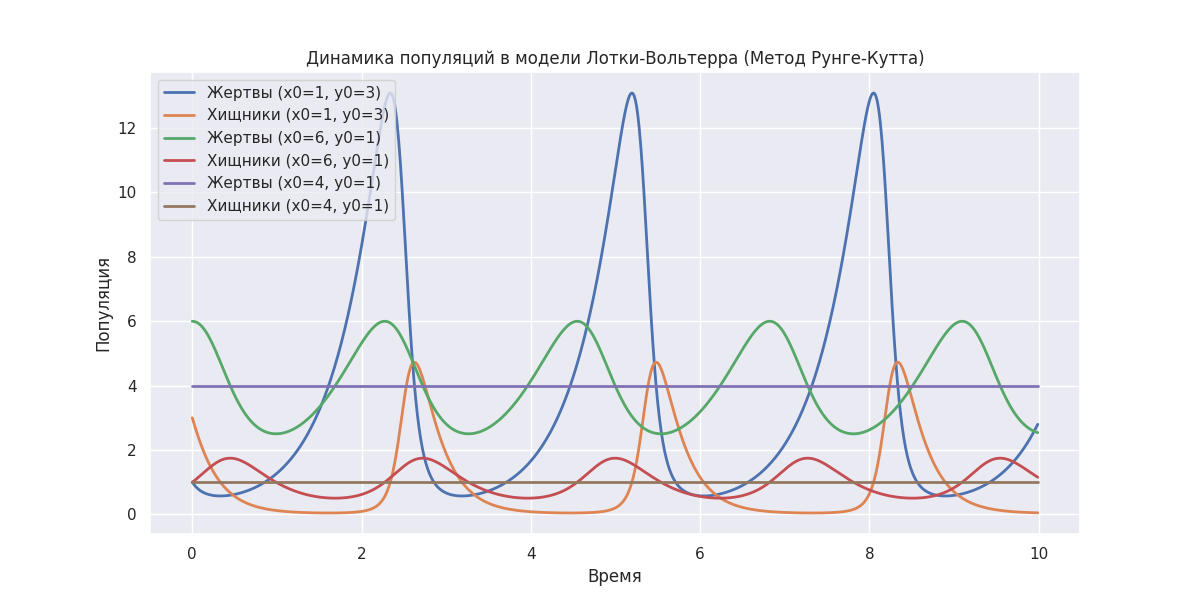
\includegraphics[width=1\textwidth]{imgs/pop_1.png}  % Вставка изображения
	\caption{Моделирование для начальных условий: $(1,3), (6,1),(4,1)$ - на временном интервале $[0,10]$ с шагом 0.01.}  % Подпись к изображению
	\label{fig:pop_1}  % Метка для ссылки
\end{figure}

Как можно видеть на (Рис. \ref{fig:pop_1}) объёмы популяций представляют собой периодические функции. Популяции взаимодействуют ровно так, как мы описали в (\ref{eq:model}). При начальном значении $(4,1)$ - популяции не изменяются.
Заметим, что некоторые популяции достигают нулевых значений. С точки зрения реального мира в эта модель будет неточной, т.к. нулевые значения у жертв вызовут вымирание обеих популяций.

Посмотрим на решение в фазовой плоскости $(x,y)$.
\begin{figure}[h]  % Окружение для картинки
	\centering
	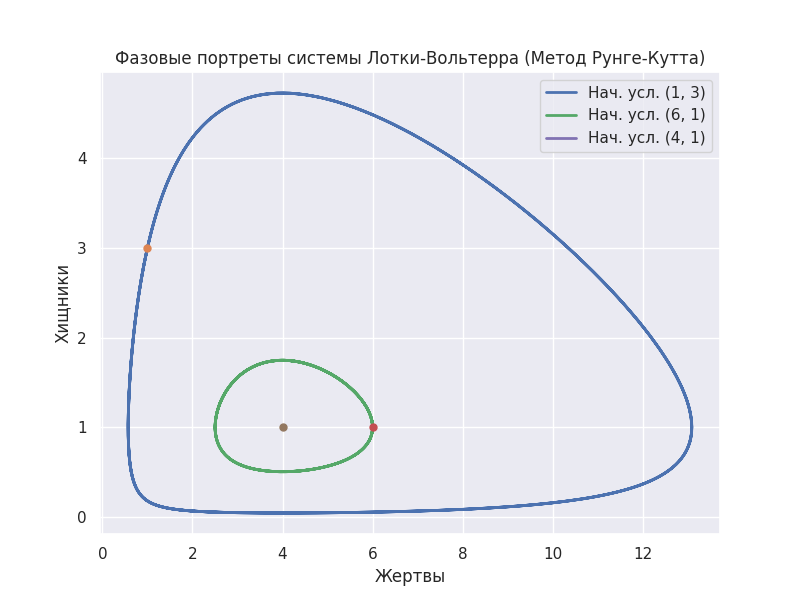
\includegraphics[width=1\textwidth]{imgs/phase_1.png}  % Вставка изображения
	\caption{Решения с начальными условиями: $(1,3)\text{ - синий}, (6,1)\text{ - зелёный}, (4,1)\text{ - коричневый}, $ - на временном интервале $[0,10]$ с шагом 0.01.}  % Подпись к изображению
	\label{fig:phase_1}  % Метка для ссылки
\end{figure}

Точками на рис. \ref{fig:phase_1} указаны начальные условия. Центральная синяя точка - положение равновесия. Как было выяснено при анализе модели, точка равновесия является неасимптотически устойчивой. Поэтому можно наблюдать циклы на фазовой плоскости. Это также было определено из первого интеграла (\ref{eq:first_int}) системы уравнений.

Уменьшим временной интервал до $[0,1]$ и шаг до 0,001, чтобы циклы не замкнулись.
\begin{figure}[h]  % Окружение для картинки
	\centering
	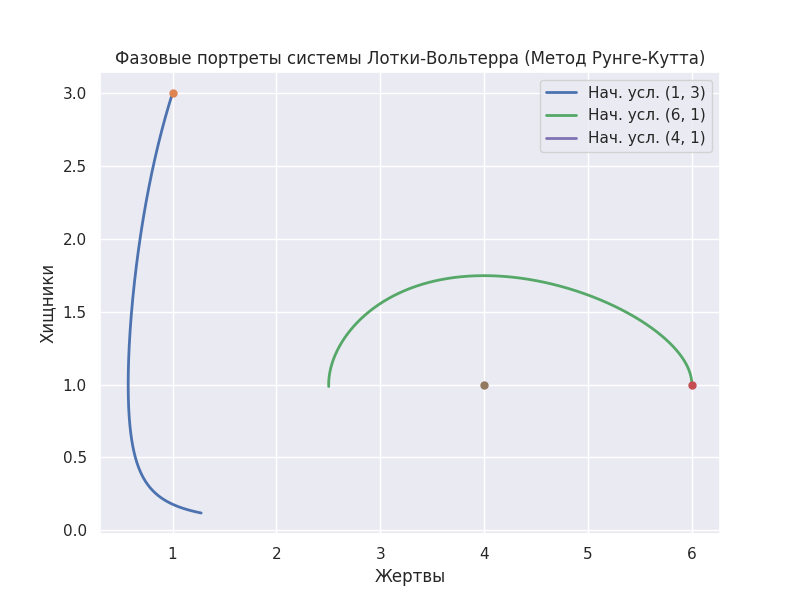
\includegraphics[width=1\textwidth]{imgs/phase_1_1.png}  % Вставка изображения
	\caption{Решения с начальными условиями: $(1,3)\text{ - синий}, (6,1)\text{ - зелёный}, (4,1)\text{ - коричневый}, $ - на временном интервале $[0,1]$.}  % Подпись к изображению
	\label{fig:phase_1_1}  % Метка для ссылки
\end{figure}

Как видно на Рис. \ref{fig:phase_1_1} циклы оставлись незамкнутыми. Кроме того, можно видеть, что они изменяются по направлению против часовой стрелки в данной фазовой плоскости.

Увеличить количество начальных параметров, чтобы увидеть действие седловой точки. Также, изменим параметры.
\newpage
\subsection*{Эксперимент 2}
Для второго эксперимента были взяты следующие параметры: $$\alpha = 2, \ \beta = 1, \ \delta = 0.1, \ \gamma = 0.8.$$

\begin{figure}[h]  % Окружение для картинки
	\centering
	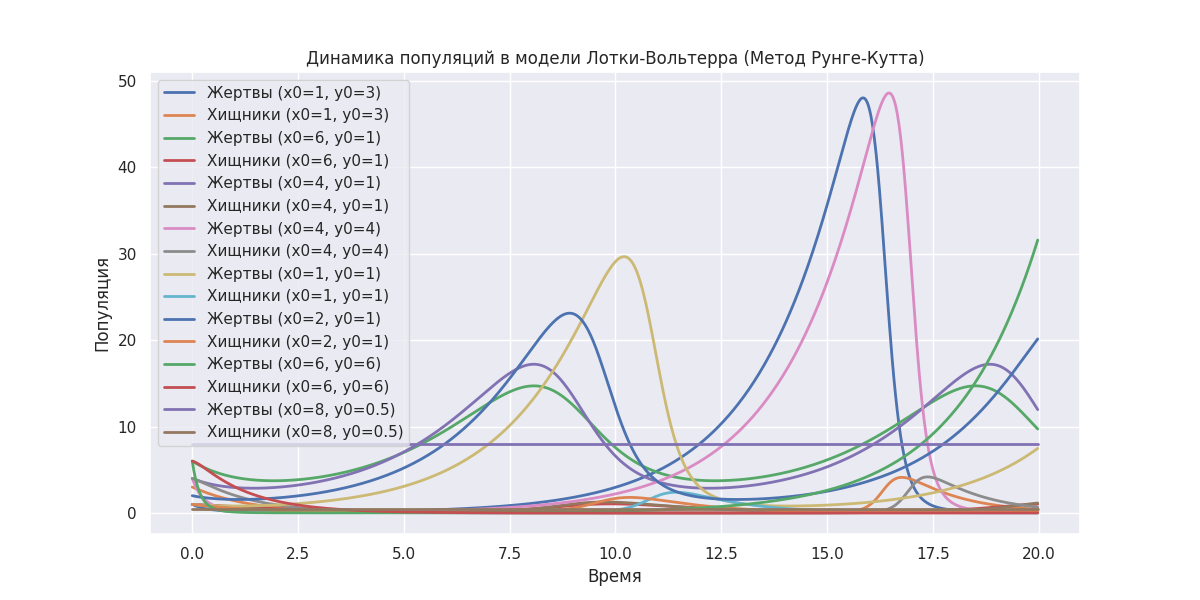
\includegraphics[width=1\textwidth]{imgs/pop_2.png}  % Вставка изображения
	\caption{Моделирование для начальных условий: $(6, 1), (5,1.3), (2,1), (8,2) = (x_{bal}, y_{bal})$.}  % Подпись к изображению
	\label{fig:pop_2}  % Метка для ссылки
\end{figure}

Заметим, что (рис. \ref{fig:pop_2}) с уменьшением коэффициентов, модель стала более "плавной". Изменение числа популяций происходит медленнее, по сравнению с прошлыми результатами. 

Кроме того, видно, что некоторые популяции приближаются к вымиранию. В реальном мире, подобный случай стал бы критическим для популяции жертв и хищников.

\begin{figure}[h]  % Окружение для картинки
	\centering
	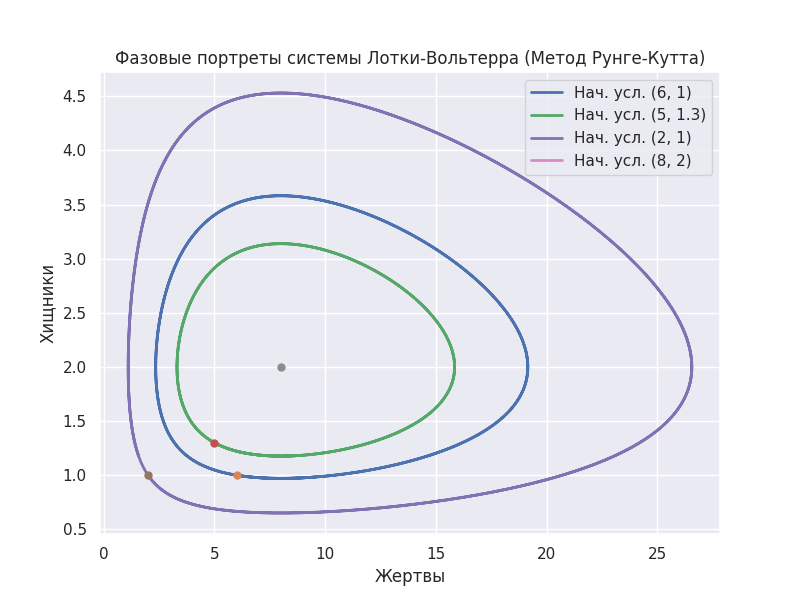
\includegraphics[width=1\textwidth]{imgs/phase_2.png}  % Вставка изображения
	\caption{Решения с указанными начальными условиями на временном интервале $[0,10]$.}  % Подпись к изображению
	\label{fig:phase_2}  % Метка для ссылки
\end{figure}

На фазовой плоскости Рис. \ref{fig:phase_2} видно, что на рассматриваемом временном интервале замкнулись не все циклы. 
Это связано с тем, что некоторые популяции достигают крайне малых значений. И для возвращения на прежний уровень требуется больше времени.

Кроме того, рис. \ref{fig:phase_2} демонстрирует свойство седловой точки. Т.к. движение по плоскости происходит против часовой стрелки, то по оси хищников движение будет происходить к началу координат (как и было получено при анализе: $\lambda_2 < 0$), не пересекая ось хищников. Аналогично и для оси жертв - движение от начала координат ($\lambda_1 > 0$).